\documentclass[../report]{subfiles}
\graphicspath{{figures/}{../figures/}}



\begin{document}

接下来测试自动机的运算,
对于%
\cref{fig:basic_a}%
的自动机$N_1$
% \cref{fig:basic_a}
\begin{figure}[H]
  \subfloat[][$N_1$]{
    \centering
    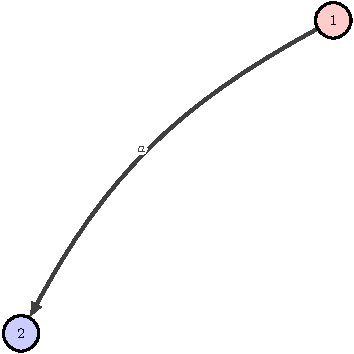
\includegraphics[width = 0.3\textwidth]{basic_a}
    \label{fig:basic_a}
  }
  \qquad
  \subfloat[][$N_2$]{
    \centering
    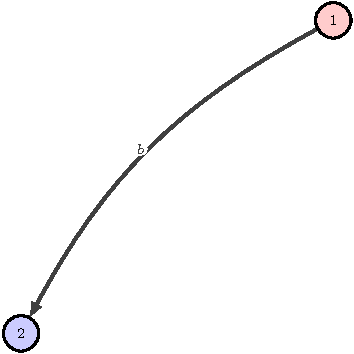
\includegraphics[width = 0.3\textwidth]{basic_b}
    \label{fig:basic_b}
  }
  %\missingfigure{basic_a}
  \caption{简单的自动机}
  \label{fig:basic}
\end{figure}

根据%
\cref{alg:star}
测试$\func{star}(N(s))$
结果如%
% \cref{fig:test_star}
\begin{figure}[H]
  \centering
  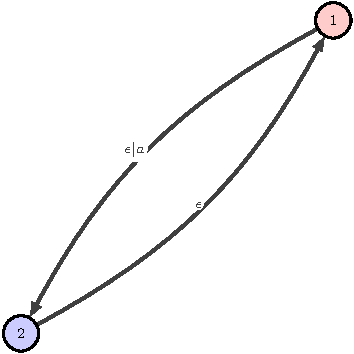
\includegraphics[width = 0.4\textwidth]{test_star}
  %\missingfigure{test_star}
  \caption{star运算测试结果}
  \label{fig:test_star}
\end{figure}

接下来完成%
\cref{alg:union}
并测试$N(s),N(t)$
如%
\cref{fig:test_union}

\begin{figure}[H]
  \centering
  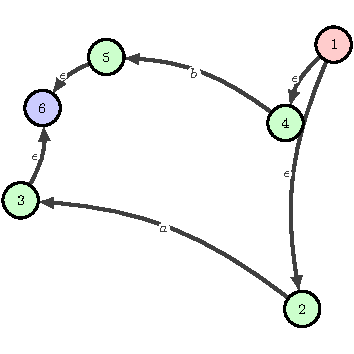
\includegraphics[width = 0.3\textwidth]{test_union}
  %\missingfigure{test_union}
  \caption{union 运算测试}
  \label{fig:test_union}
\end{figure}

最后根据%
\cref{alg:concatenation}
完成concatenation运算代码并绘图,得
% \cref{fig:test_concatenation}
\begin{figure}[H]
  \centering
  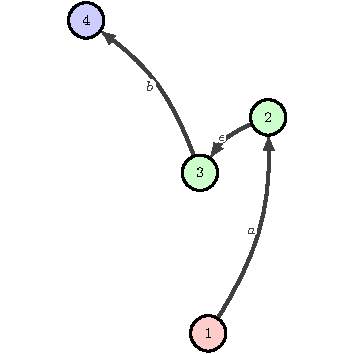
\includegraphics[width = 0.4\textwidth]{test_concatenation}
  %\missingfigure{test_concatenation}
  \caption{concatenation$(N(s),N(t))$的结果}
  \label{fig:test_concatenation}
\end{figure}


\end{document}
